%%% Template originaly created by Karol Kozioł (mail@karol-koziol.net) and modified for ShareLaTeX use

%%%------------------------------------------------------------------------------------------------%%%
%%%------------------------------------%%%     PREAMBLE     %%%------------------------------------%%%
%%%------------------------------------------------------------------------------------------------%%%

\documentclass[twoside=false,a4paper,11pt]{article}

\usepackage[T1]{fontenc}
\usepackage[utf8]{inputenc}
\usepackage{graphicx}
\usepackage{xcolor}

\usepackage{tgtermes}



\usepackage[
pdftitle={CPSC 471 Final Report}, 
pdfauthor={Timothy Mealey, University of Calgary},
colorlinks=true,linkcolor=blue,urlcolor=blue,citecolor=blue,bookmarks=true,
bookmarksopenlevel=2]{hyperref}
\usepackage{amsmath,amssymb,amsthm,textcomp}

\usepackage{enumitem}

\usepackage{multicol}
\usepackage{tikz}
\usetikzlibrary{shapes,positioning,calc}
\colorlet{lightgray}{gray!20}

\usepackage{geometry}
\geometry{total={210mm,297mm},
left=25mm,right=25mm,%
bindingoffset=0mm, top=20mm,bottom=20mm}

\linespread{1.3}

\newcommand{\linia}{\rule{\linewidth}{0.5pt}}

% custom theorems if needed
\newtheoremstyle{mytheor}
    {1ex}{1ex}{\normalfont}{0pt}{\scshape}{.}{1ex}
    {{\thmname{#1 }}{\thmnumber{#2}}{\thmnote{ (#3)}}}

\theoremstyle{mytheor}
\newtheorem{defi}{Definition}

% my own titles
\makeatletter
\renewcommand{\maketitle}{
\begin{center}
\vspace{2ex}
{\huge \textsc{\@title}}
\vspace{1ex}
\\
\linia\\
\@author \hfill \@date
\vspace{4ex}
\end{center}
}
\makeatother
%%%

% custom footers and headers
\usepackage{fancyhdr,lastpage}
\pagestyle{fancy}
\lhead{}
\chead{}
\rhead{}
\lfoot{Final Report}
\cfoot{}
\rfoot{Page \thepage\ /\ \pageref*{LastPage}}
\renewcommand{\headrulewidth}{0pt}
\renewcommand{\footrulewidth}{0pt}
%


%%%------------------------------------------------------------------------------------------------%%%
%%%------------------------------------%%%     DOCUMENT     %%%------------------------------------%%%
%%%------------------------------------------------------------------------------------------------%%%

\newcommand{\tuple}[2]{\{ #1 | #2 \}}
\newcommand{\domain}[2]{\{ (#1) | #2 \}}

\newcommand{\quantifier}[2]{(\ensuremath{#1}#2)}
\newcommand{\one}[1]{\quantifier{\exists}{#1}}
\newcommand{\all}[1]{\quantifier{\forall}{#1}}

\begin{document}

\title{CPSC 471 Final Report}
\author{Timothy Mealey, Ben Roberts, Cory Jensen, Scott Saunders}
\date{\today}
\maketitle

\section*{Abstract}

``An abstract of no more than 300 words.''

\section*{Introduction}

``Describe the problem or task your database was designed to address.
Describe (briefly) the system you have created to address the problem or task.''

\section*{Design}

\subsection*{Users}

``Discuss the different users of your system. Your discussion in this section should be considerably more detailed than what you described for the presentation - this section should describe a complete transaction collection and, consequently, provide a complete picture of the functionality offered by your system.''

\subsubsection*{Log In}
\subsubsection*{Course Search}
\subsubsection*{Schedule Creator}

\subsection*{Entity Relationship Diagram}

\includegraphics[width=\textwidth]{ERDiagram.png}

``Any changes that were made since the presentation should be clearly indicated.''

\section*{Implementation}

\subsection*{Relational Schema Diagram}

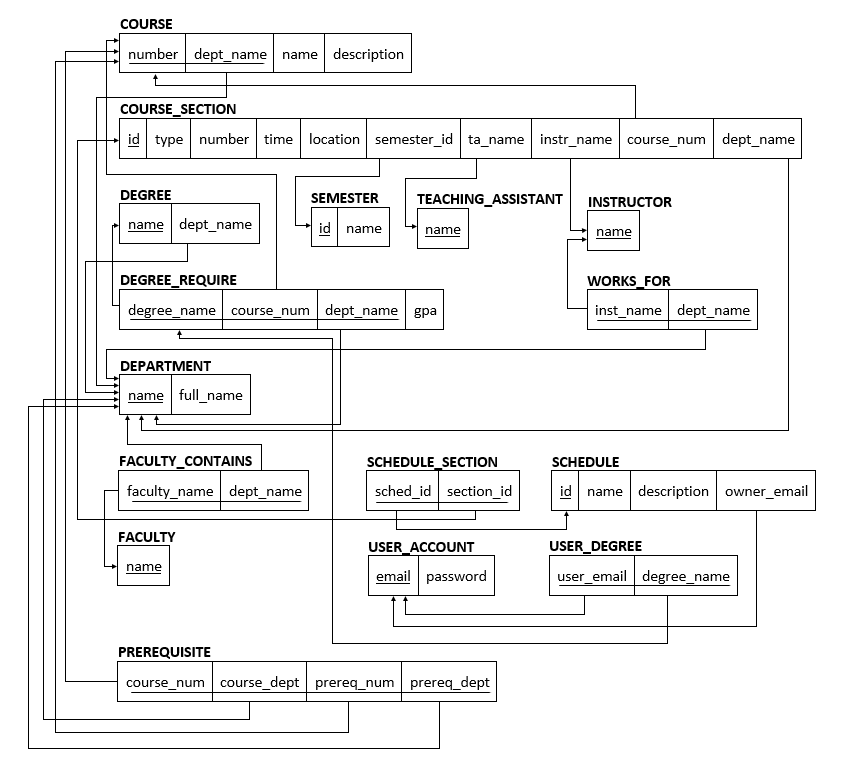
\includegraphics[width=\textwidth]{RelationalSchemaDiagram.png}

``Discuss any significant or unusual decisions made during this process.''

\subsection*{Database Management System}

``Describe the DBMS you selected for the implementation	of the project, and include the SQL statements for each of the transactions implemented. It is not necessary to discuss these transactions in relational algebra or calculus.''

\subsection*{User Interface}

``Present a brief description of your interface design, including several screenshots.''

\end{document}